\documentclass[11pt,letterpaper]{article}
\usepackage[T1]{fontenc}
\usepackage[scaled]{helvet}
\renewcommand{\familydefault}{\sfdefault}
\usepackage{amsmath,amssymb}
\usepackage[margin=0.8in,bottom=0.9in]{geometry}
\usepackage[most]{tcolorbox}
\usepackage{tikz}
\usetikzlibrary{calc}
\usepackage{enumitem}
\usepackage{array}
\usepackage{needspace}
\usepackage{fancyhdr}
\usepackage{pifont}

% ---- Palette "F. Bright & Playful" ----
\definecolor{fmtitle}{HTML}{3D2C8D}
\definecolor{fmkey}{HTML}{0096C7}
\definecolor{fmwatch}{HTML}{2BB673}
\definecolor{fmturn}{HTML}{F4A100}
\definecolor{fmmistake}{HTML}{EF476F}
\definecolor{fmnotice}{HTML}{9B5DE5}
\definecolor{fmgray}{HTML}{6B6B6B}

\pagestyle{fancy}
\fancyhf{}
\renewcommand{\headrulewidth}{0pt}
\fancyfoot[C]{\footnotesize\color{fmgray}\textcopyright\ 2026 FangMath. All rights reserved.}
\fancyfoot[R]{\footnotesize\color{fmgray}\thepage}
\setlength{\parindent}{0pt}
\setlength{\parskip}{3pt}

\newcommand{\badge}[1]{\colorbox{fmtitle}{\color{white}\bfseries\small\ #1\ }}
\newcommand{\leveltag}[2]{\colorbox{#1}{\color{white}\bfseries\scriptsize\ #2\ }}
\newcommand{\LE}{\leveltag{fmwatch}{EASY}}
\newcommand{\LM}{\leveltag{fmturn}{MEDIUM}}
\newcommand{\LH}{\leveltag{fmmistake}{HARD}}

\newcommand{\sectionbar}[2]{\needspace{6cm}\par\vspace{4mm}
  \begin{tcolorbox}[enhanced,colback=fmtitle,colframe=fmtitle,arc=2mm,
    left=4mm,top=1.5mm,bottom=1.5mm]
  \color{white}\bfseries\large #1\hfill{\normalsize\mdseries #2}
  \end{tcolorbox}}

\newtcolorbox{keyidea}{enhanced,breakable,colback=white,colframe=fmkey,boxrule=1pt,arc=2mm,
  title={Key Idea},coltitle=fmkey,fonttitle=\bfseries,
  attach boxed title to top left={xshift=4mm,yshift=-2mm},
  boxed title style={colback=white,colframe=fmkey,boxrule=0.9pt}}
\newtcolorbox{watchme}{enhanced,colback=white,colframe=fmwatch,boxrule=1pt,arc=2mm,
  title={Watch Me --- Worked Example},coltitle=fmwatch,fonttitle=\bfseries,
  attach boxed title to top left={xshift=4mm,yshift=-2mm},
  boxed title style={colback=white,colframe=fmwatch,boxrule=0.9pt}}
\newtcolorbox{mistakebox}{enhanced,breakable,colback=white,colframe=fmmistake,boxrule=1pt,arc=2mm,
  title={Common Mistake},coltitle=fmmistake,fonttitle=\bfseries,
  attach boxed title to top left={xshift=4mm,yshift=-2mm},
  boxed title style={colback=white,colframe=fmmistake,boxrule=0.9pt}}
\newtcolorbox{yourturn}{enhanced,breakable,colback=white,colframe=fmturn,boxrule=1pt,arc=2mm,
  title={Your Turn},coltitle=fmturn,fonttitle=\bfseries,
  attach boxed title to top left={xshift=4mm,yshift=-2mm},
  boxed title style={colback=white,colframe=fmturn,boxrule=0.9pt}}
\newtcolorbox{answerbox}[1]{enhanced,breakable,colback=white,colframe=fmwatch,boxrule=1pt,arc=2mm,
  title={#1},coltitle=fmwatch,fonttitle=\bfseries,
  attach boxed title to top left={xshift=4mm,yshift=-2mm},
  boxed title style={colback=white,colframe=fmwatch,boxrule=0.9pt}}

\newcommand{\work}[1]{\par\vspace{#1}}
\setlist[enumerate]{itemsep=2pt,topsep=3pt}

% ---------------- extra boxes ----------------
\newtcolorbox{notebox}{enhanced,breakable,colback=white,colframe=fmnotice,boxrule=1pt,arc=2mm,
  title={Notice},coltitle=fmnotice,fonttitle=\bfseries,
  attach boxed title to top left={xshift=4mm,yshift=-2mm},
  boxed title style={colback=white,colframe=fmnotice,boxrule=0.9pt}}
\newtcolorbox{exbox}{enhanced,colback=white,colframe=fmwatch,boxrule=0.8pt,arc=2mm,
  title={Example},coltitle=fmwatch,fonttitle=\bfseries\small,
  attach boxed title to top left={xshift=4mm,yshift=-2mm},
  boxed title style={colback=white,colframe=fmwatch,boxrule=0.8pt},fontupper=\small}
\newcommand{\topicbar}[1]{\needspace{4.5cm}\par\vspace{5mm}
  \begin{tcolorbox}[enhanced,colback=fmtitle,colframe=fmtitle,arc=2mm,left=4mm,top=1.5mm,bottom=1.5mm]
  \color{white}\bfseries\large #1
  \end{tcolorbox}}
\usepackage{multicol}

% ---------------- practice layout ----------------
\newcommand{\workline}{\par\vspace{7mm}{\color{gray!55}\rule{\linewidth}{0.4pt}}}
\newcommand{\worklines}[1]{\foreach \i in {1,...,#1}{\workline}}
\newcommand{\prob}[3]{\needspace{#3}\par\vspace{3mm}{\color{fmturn}\bfseries #1.}\ #2\par}
\newcommand{\ansline}{\par\vspace{4mm}\hfill\textbf{Answer:}\ \rule{5cm}{0.4pt}\par}
\newcommand{\keyitem}[3]{\needspace{3.2cm}\par\vspace{2mm}
  \begin{tcolorbox}[enhanced,colback=white,colframe=fmwatch!60,boxrule=0.6pt,arc=1.5mm,left=3mm,top=1.5mm,bottom=1.5mm]
  {\color{fmwatch}\bfseries #1.}\quad\small #2\par\vspace{1mm}
  \normalsize\textbf{Answer: #3}
  \end{tcolorbox}}


\usetikzlibrary{arrows.meta}
\providecommand{\iskey}{0}
% fill-in blank: line for students, pink answer in the key
\newcommand{\fb}[2][2.6cm]{\ifnum\iskey=1 \underline{\makebox[#1][c]{\color{fmmistake}\bfseries #2}}\else\underline{\makebox[#1]{}}\fi}
% answer line for practice problems
\newcommand{\pans}[2][3.2cm]{\ifnum\iskey=1 \underline{\makebox[#1][c]{\color{fmmistake}\bfseries #2}}\else\rule{#1}{0.4pt}\fi}
\newcommand{\vid}[1]{{\color{fmgray}\small\textit{\ding{43} Video: #1}}}
\newcommand{\pt}[2]{\fill (#1) circle (2.2pt) node[above=1pt,font=\small]{$#2$};}

\usetikzlibrary{decorations.pathreplacing}
% three points on a segment with lengths written above the pieces: #1,#2,#3 letters; #4,#5 piece labels; #6 whole label (below)
\newcommand{\threept}[6]{\begin{tikzpicture}[x=1cm]\draw[thick] (0,0)--(3.6,0);
\fill (0,0) circle(2.2pt) node[below=2pt,font=\small]{$#1$} (1.4,0) circle(2.2pt) node[below=2pt,font=\small]{$#2$} (3.6,0) circle(2.2pt) node[below=2pt,font=\small]{$#3$};
\node[above,font=\small] at (0.7,0.02){#4};\node[above,font=\small] at (2.5,0.02){#5};
\if\relax\detokenize{#6}\relax\else\draw[gray,decorate,decoration={brace,amplitude=4pt,mirror}] (0,-0.45)--(3.6,-0.45) node[midway,below=4pt,font=\small]{#6};\fi
\end{tikzpicture}}
\newcommand{\sdp}[3]{\begin{minipage}[t][2.4cm]{0.48\linewidth}{\color{fmturn}\bfseries #1.}\ #2\par\vfill\hfill \pans[3.6cm]{#3}\end{minipage}}
\newcommand{\figp}[4]{\begin{minipage}[t]{0.48\linewidth}{\color{fmturn}\bfseries #1.}\ #2\par\vspace{1mm}\centering #3\par\vspace{2mm}\raggedleft \pans[2.6cm]{#4}\end{minipage}}
\newcommand{\algp}[3]{\begin{minipage}[t][4.6cm]{0.48\linewidth}{\color{fmturn}\bfseries #1.}\ #2\par\vfill\hfill \pans[4.2cm]{#3}\end{minipage}}


% ch2: long key answers wrap inside their column instead of running into the next one
\newlength{\pw}
\renewcommand{\pans}[2][3.2cm]{\ifnum\iskey=1 \settowidth{\pw}{\bfseries #2}\ifdim\pw>#1 \parbox[b]{#1}{\raggedleft\color{fmmistake}\bfseries\small #2}\else\underline{\makebox[#1][c]{\color{fmmistake}\bfseries #2}}\fi\else\rule{#1}{0.4pt}\fi}
\begin{document}
\ifnum\iskey=1 \colorbox{fmwatch}{\color{white}\bfseries\small\ ANSWER KEY\ }\else\badge{PRACTICE}\fi\hfill{\small\color{fmgray}Geometry \textperiodcentered\ Lesson 2.6}\par\vspace{4mm}
{\color{fmtitle}\LARGE\bfseries Proving Angle Relationships --- Practice\ifnum\iskey=1 \ --- Answer Key\fi}\par\vspace{1mm}
{\color{fmgray}A worked example comes before each type. Show your thinking.}\par\vspace{3mm}
Name: \rule{6cm}{0.4pt}\hspace{1cm}Date: \rule{3.5cm}{0.4pt}\par\vspace{2mm}
\newcommand{\Xfig}{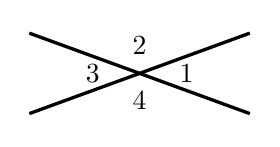
\begin{tikzpicture}[scale=0.7]\draw[very thick] (-2,-0.73)--(2,0.73); \draw[very thick] (-2,0.73)--(2,-0.73); \node at (0.85,0){$1$}; \node at (0,0.5){$2$}; \node at (-0.85,0){$3$}; \node at (0,-0.5){$4$};\end{tikzpicture}}
\newcommand{\rsn}[1]{\pans[6.2cm]{#1}}

\needspace{6cm}\topicbar{Type 1 \quad Vertical Angles and Linear Pairs}
\begin{watchme}\begin{minipage}[c]{0.26\linewidth}\centering\Xfig\end{minipage}\hfill
\begin{minipage}[c]{0.7\linewidth}$m\angle 1 = 48^\circ$. \ $\angle 3$ is vertical to $\angle 1$: $m\angle 3 = 48^\circ$.\par
$\angle 2$ and $\angle 1$ are a linear pair: $m\angle 2 = 180^\circ - 48^\circ = 132^\circ$; \ $m\angle 4 = 132^\circ$ (vertical to $\angle 2$).\end{minipage}\end{watchme}
\needspace{3.4cm}\noindent\sdp{1}{Use the figure above. $m\angle 2 = 115^\circ$. Find $m\angle 4$.}{$115^\circ$}\hfill\sdp{2}{$m\angle 2 = 115^\circ$. Find $m\angle 1$.}{$65^\circ$}\par\vspace{2mm}
\needspace{3.4cm}\noindent\sdp{3}{$m\angle 3 = 72^\circ$. Find $m\angle 1$, $m\angle 2$ and $m\angle 4$.}{$72^\circ,\ 108^\circ,\ 108^\circ$}\hfill\sdp{4}{Are $\angle 1$ and $\angle 2$ vertical angles or a linear pair?}{a linear pair}\par

\needspace{6cm}\topicbar{Type 2 \quad Solve With Algebra}
\begin{watchme}$m\angle 1 = 4x + 6$ and $m\angle 3 = 6x - 14$ (vertical angles). \ $4x + 6 = 6x - 14 \Rightarrow 20 = 2x \Rightarrow x = 10$.\par
$m\angle 1 = 4(10) + 6 = 46^\circ$. \quad \textbf{Answer: $\boldsymbol{x = 10,\ m\angle 1 = 46^\circ}$}\end{watchme}
\needspace{4.6cm}\noindent\algp{5}{$m\angle 1 = 5x - 12$, $m\angle 3 = 3x + 20$. Find $x$ and $m\angle 1$.}{$x = 16$, $m\angle 1 = 68^\circ$}\hfill\algp{6}{$m\angle 1 = 2x + 10$, $m\angle 2 = 4x - 10$ (linear pair). Find $x$ and $m\angle 2$.}{$x = 30$, $m\angle 2 = 110^\circ$}\par\vspace{2mm}
\needspace{4.6cm}\noindent\algp{7}{$\angle A$ and $\angle B$ are both complementary to $\angle C$. $m\angle A = 3x - 4$, $m\angle B = x + 20$. Find $m\angle A$.}{$x = 12$, $m\angle A = 32^\circ$}\hfill\algp{8}{\LH\ $m\angle 1 = x^2$, $m\angle 3 = 5x + 14$ (vertical angles), $x > 0$. Find $m\angle 1$.}{$x = 7$, $m\angle 1 = 49^\circ$}\par

\needspace{8cm}\topicbar{Type 3 \quad Complete the Proof}
\begin{watchme}Given: $\angle 1$ and $\angle 2$ are right angles. \ Prove: $\angle 1 \cong \angle 2$.\par
1.\ $\angle 1$ and $\angle 2$ are right angles (Given) \quad 2.\ $\angle 1 \cong \angle 2$ (Right Angles Congruence Theorem)\end{watchme}
\needspace{6cm}{\color{fmturn}\bfseries 9.}\ \begin{minipage}[t]{0.62\linewidth}Given: two lines intersect, forming $\angle 1$--$\angle 4$ as in the Type 1 figure. \ Prove: $\angle 2 \cong \angle 4$.\end{minipage}
\par\vspace{1mm}\renewcommand{\arraystretch}{1.9}\begin{tabular}{@{}p{6.2cm}|l@{}}\textbf{Statements} & \textbf{Reasons}\\ \hline
1.\ $\angle 2$ and $\angle 4$ are vertical angles & \rsn{Definition of vertical angles}\\
2.\ $\angle 2 \cong \angle 4$ & \rsn{Vertical Angles Congruence Theorem}\\
\end{tabular}\par\vspace{3mm}
\needspace{6cm}{\color{fmturn}\bfseries 10.}\ Given: $\angle 1$ and $\angle 2$ are a linear pair, and $\angle 2$ and $\angle 3$ are a linear pair. \ Prove: $\angle 1 \cong \angle 3$.
\par\vspace{1mm}\begin{tabular}{@{}p{6.2cm}|l@{}}\textbf{Statements} & \textbf{Reasons}\\ \hline
1.\ $\angle 1, \angle 2$ and $\angle 2, \angle 3$ are linear pairs & Given\\
2.\ $\angle 1, \angle 2$ supplementary; $\angle 2, \angle 3$ supplementary & \rsn{Linear Pair Postulate}\\
3.\ $\angle 1 \cong \angle 3$ & \rsn{Congruent Supplements Theorem}\\
\end{tabular}\par

\needspace{5cm}\topicbar{Type 4 \quad Always, Sometimes or Never?}
\begin{watchme}``Two angles that form a linear pair are congruent.'' \ Only when both are $90^\circ$. \quad \textbf{Answer: sometimes.}\end{watchme}
\needspace{3.4cm}\noindent\sdp{11}{Vertical angles are congruent.}{always}\hfill\sdp{12}{Two right angles are supplementary.}{always}\par\vspace{2mm}
\needspace{3.4cm}\noindent\sdp{13}{Two supplementary angles are both acute.}{never}\hfill\sdp{14}{\LH\ Two angles complementary to the same angle are congruent.}{always}\par
\end{document}
